\documentclass[tikz,border=2pt]{standalone}
\usepackage{amsmath}
\usepackage{tikz}

\begin{document}
% 1+2+...+n as a staircase: two copies fit together into an n x (n+1) rectangle, so the sum is n(n+1)/2.
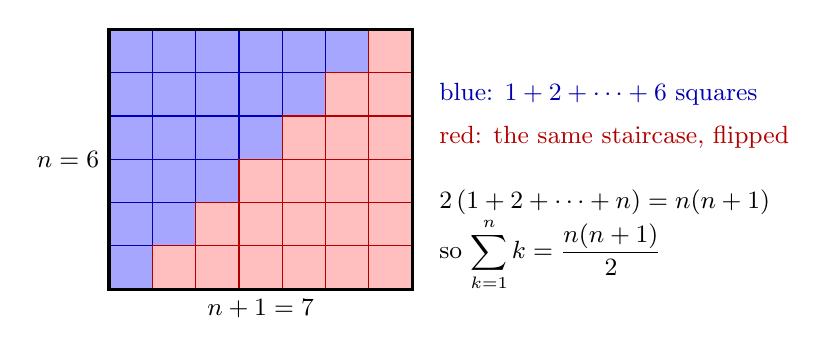
\begin{tikzpicture}[scale=0.55, every node/.style={font=\small}]
	\foreach \i in {1,...,6} {
		\foreach \j in {1,...,\i} {\fill[blue!35, draw=blue!70!black] (\j-1,\i-1) rectangle (\j,\i);}
	}
	\foreach \i in {1,...,6} {
		\foreach \j in {\i,...,6} {\fill[red!25, draw=red!70!black] (\j,\i-1) rectangle (\j+1,\i);}
	}
	\draw[very thick] (0,0) rectangle (7,6);
	\node[below] at (3.5,0) {$n+1=7$};
	\node[left] at (0,3) {$n=6$};
	\node[blue!70!black, anchor=west] at (7.4,4.5) {blue: $1+2+\cdots+6$ squares};
	\node[red!70!black, anchor=west] at (7.4,3.5) {red: the same staircase, flipped};
	\node[anchor=west] at (7.4,2.0) {$2\,(1+2+\cdots+n)=n(n+1)$};
	\node[anchor=west] at (7.4,0.8) {so $\displaystyle\sum_{k=1}^{n}k=\frac{n(n+1)}2$};
\end{tikzpicture}
\end{document}
